\documentclass[ex, minted]{exercise_4.0}

\deadline{15.05.2024}

\begin{document}

\section{Stern-Gerlach Experiment}
{\it Mit einem Atomstrahl aus Kalium-Atomen wird ein Stern-Gerlach-Experiment durchgeführt. Die Temperatur des Ofens beträgt $T = 190^\circ \mathrm C ,$ das Magnetfeld besitzt eine Inhomogenität $\pp Bz = 82  \ufrac Tm$. Die Atome
durchfliegen das Magnetfeld auf einer Strecke von $l = 10 \u{cm}$. In einem Abstand von $d = 32 \u{cm}$ hinter dem Magneten befindet sich eine Glasplatte, auf der die Atome aufgefangen werden.}

\subsection
{\it In welchem mittleren Abstand in $z$-Richtung beobachtet man die beiden Atomstrahlen auf der Glasplatte (siehe Abbildung)? \\
Hinweis: Bei Kalium trägt nur der Spin des Elektrons im $4^2s_{1/2}$ Zustand bei.}

\dottedlinett

Für die mittlere Geschwindigkeit der Teilchen beim Austritt aus dem Ofen gilt:
\begin{align*}
    \tug{E\sub T} &= \tug{E\sub{kin}}\\ 
    \frac32 k_B  T &= \frac12 m \tug{v_x^2} \\ 
    \tug{v_x^2} &= 3 k_B /m T \\ 
    \tug{v_x} &\approx  \sqrt{3 k_B /m T} \\
    &\approx  522\ufrac ms  \with  m = 39\E{-3} /n_A \\
\end{align*}

Sind die Teilchen ins B-Feld eingetreten, wirkt auf sie die Kraft:
\begin{align*}
    \v F &= -\grad V\\
    &= -\grad (-\v \mu \cdot \v B)\\
    &= \mu_z \,\pp{\v B}z \cdot  \e_z\\
\end{align*}
Bei verlassen des B-Feldes ergeben sich damit folgende Position und Geschwindigkeit:
\begin{align*}
    v_z &= a t\\
    &=  \frac{F_z l}{m v_x}\\ 
    &=  \frac{\mu_z \,l}{m v_x} \pp{\v B}z\\ 
    &\approx 2.25 \ufrac ms\\
    \\
    z' &= \frac 12 a t^2\\
    &= \frac 12 \frac{F}{m} \hug{\frac{l}{v_x}}^2\\
    &= \frac 12 \frac{\mu_z l^2}{m v_x^2} \pp{\v B}z \\
\end{align*} 

Auf der Strecke zwischen B-Feld und Schirm, wirken keine Kräfte und die Teilchen bewegen sich geradlinig gleichförmig. Damit ergibt sich der mittlere Abstand auf der Glasplatte \(z''\) als:
\begin{align*}
    z'' &= z' + v_z t\\
    &= z' + d \frac{v_z }{v_x}\\
    &= \frac 12 \frac{\mu_z l^2}{m v_x^2} \pp{\v B}z + d \frac{v_z }{v_x}\\
    &= \frac 12 \frac{\frac12 g_s \mu_B \cdot l^2}{m v_x^2} \pp{\v B}z + d \frac{v_z }{v_x}\\
    &\approx 1.38\u{mm}
\end{align*}


\subsection
{\it Entwickeln Sie ein python-Skript oder Jupyter-Notebook mit einer Monte Carlo Simulation des Stern-Gerlach Experiments mit der Sie den Auftreffort einzelner Kalium-Atome darstellen können. Würfeln
Sie dazu zunächst die inertialen Teilchengeschwindigkeiten, die einer Maxwell-Boltzmann-Verteilung mit
der gegebenen Temperatur folgen.
Nutzen Sie diese dann, um die Verteilung der Kalium-Atome am Schirm als Histogramm darzustellen.
Nehmen Sie an, dass das Experiment unter perfekten Laborbedingungen stattfindet, das Experiment also
durch die gegebenen Parameter und die Abbildung vollständig beschrieben wird. Es darf angenommen
werden, dass Teilchen aus dem Kollimator an immer exakt der gleichen Position und mit exakt gleicher
Flugrichtung austreten. Sie können ebenfalls einen Gangunterschied im Magnetfeld vernachlässigen.
Vergleichen Sie die Verteilung mit Ihrer Erwartung aus Aufgabenteil (a).\\
Tipp: Verwenden Sie zum generieren von Zufallszahlen in ihrer Monte Carlo Simulation geeignete Pseudozufallszahlengeneratoren wie z.B. numpy.random.uniform in Python.}

\dottedlinett

\inputpy{Python-Code}{5.py}

\begin{figure}[H]
    \centering
    \includesvg[width=\textwidth]{5.svg}
    \caption{resultierender Plot}
\end{figure}

Wie man sieht, trifft der errechnete Wert für \(z''\) gut den Wert höhster Wahrscheinlichkeit. Jedoch ist der mittlere Wert für \(z''\) etwa um ein vierfaches größer, da die Verteilung \(p(z'')\) für \(z''\to\inf\) nur langsam abfällt. 


\section{Mögliche Übergänge beim normalen Zeeman-Effekt}
\subsection{\it Schreiben Sie alle möglichen Dipolübergänge zwischen dem d-Niveau in ein p-Niveau in der Standardnomenklatur auf.}

\dottedlinett

Prinzipiell gibt es folgende Übergänge  (mit \(\ket{l,m_l}\) und \((\dots)\) als verschiedene seperate Möglichkeiten):
\begin{align*}
    \ket{3, \pm(0,1,2,3)} \to \ket{2, \pm(0,1,2)}
\end{align*}
Physikalisch sind jedoch nur die, welche die Auswahlregel \(\Delta m = 0,\pm1\) erfüllen. Damit bleiben:
\begin{align*}
    \ket{3, \pm3} &\to \ket{2, \pm2}\\
    \ket{3, \pm2} &\to \ket{2, \pm(1,2)}\\
    \ket{3, \pm1} &\to \ket{2, \pm(0,1,2)}\\
    \ket{3, 0} &\to \ket{2, \pm(0,1)}
\end{align*}
In der Standardnomenklatur:
\begin{align*}
    d_{\pm3} &\to p_{\pm2}\\
    d_{\pm2} &\to p_{\pm(1,2)}\\
    d_{\pm1} &\to p_{\pm(0,1,2)}\\
    d_0 &\to p_{\pm(0,1)}
\end{align*}

\subsection{\it Wie viele der Übergänge aus (a) unterscheiden sich energetisch? Schreiben Sie auf, welche der Übergänge aus (a) zur gleichen Spektrallinie führen.\\
Hinweis: Die Auswahlregel für die elektrischen Übergänge lautet \(\Delta m=+1,0,-1\).}

\dottedlinett

Die Spektrallinie zum Übergang \(d\to p\) spaltet sich durch den Zeeman-Effekt in drei Energieniveaus \(E_{-1,0,1}\) auf, welche den drei Möglichkeiten \(\Delta m = -1,0,1\) entsprechen:

% \begin{align*}
%     E_{-1}& \equiv \begin{cases}
%         \ket{3,3} \to \ket{2,2}\\
%         \ket{3,2} \to \ket{2,1}\\
%         \ket{3,1} \to \ket{2,0}\\
%         \ket{3,0} \to \ket{2,-1}\\
%         \ket{3,-1} \to \ket{2-2}\\
%     \end{cases}\\\\
%     E_0&\equiv  \begin{cases}
%         \ket{3,\pm2} \to \ket{2,\pm2}\\
%         \ket{3,\pm1} \to \ket{2,\pm1}\\
%         \ket{3,0} \to \ket{2,0}\\
%     \end{cases}\\\\
%     E_1 &\equiv  \begin{cases}
%         \ket{3,-3} \to \ket{2,-2}\\
%         \ket{3,-2} \to \ket{2,-1}\\
%         \ket{3,-1} \to \ket{2,0}\\
%         \ket{3,-0} \to \ket{2,1}\\
%         \ket{3,1} \to \ket{2,2}\\
%     \end{cases}\\
% \end{align*}

\begin{align*}
    E_{-1}& \equiv \begin{cases}
        d_{3} \to p_{2}\\
        d_{2} \to p_{1}\\
        d_{1} \to p_{0}\\
        d_{0} \to p_{-1}\\
        d_{-1} \to p_{-2}\\
    \end{cases}\\\\
    E_0&\equiv  \begin{cases}
        d_{\pm2} \to p_{\pm2}\\
        d_{\pm1} \to p_{\pm1}\\
        d_{0} \to p_{0}\\
    \end{cases}\\\\
    E_1 &\equiv  \begin{cases}
        d_{-3} \to p_{-2}\\
        d_{-2} \to p_{-1}\\
        d_{-1} \to p_{0}\\
        d_{-0} \to p_{1}\\
        d_{1} \to p_{2}\\
    \end{cases}\\
\end{align*}

\section{Anormaler Zeeman-Effekt}
{\it Bei Natrium tritt der anomale Zeeman-Effekt auf. Die Natrium-$D_2$-Linie ist der Übergang von $3^2P_{3/2}$ nach
$3^2S_{1/2}$.}

\subsection{\it Betrachten Sie die Aufspaltung der $D_2$-Linie in einem externen Magnetfeld $B$. In wieviele Niveaus spalten $3^2P_{3/2}$ bzw. $3^2S_{1/2}$ auf?
Wie groß ist die Aufspaltung zwischen zwei benachbarten Zeeman-Linien in Einheiten von $\mu_B B$?}

\dottedlinett

$3^2P_{3/2}$ spaltet sich auf in vier Niveaus auf \((m_j = \pm3/2, \pm1/2 )\), während 
$3^2S_{1/2}$ sich in zwei Niveaus \((m_j = \pm1/2)\) aufspaltet.

\begin{align*}
    V_B &= \mu_B B \, g_j m_j \\
    \implies \Delta V_B &= \mu_B B \, g_j \\
    \\
    g_J &= 1 +(g_S-1)\frac{j(j+1) + s(s+1) - l(l+1)}{2 j(j+1)} \\
    &\approx  1 +\frac{j(j+1) + s(s+1) - l(l+1)}{2 j(j+1)} \\
    \\
    g_J\hug{3^2P_{3/2}} &= 1 + \frac{3/2(3/2+1) + 1/2(1/2+1) - 1(1+1)}{2 \cdot 3/2(3/2+1)}\\
    &= 4/3\\
    \implies \Delta V_B\hug{3^2P_{3/2}} &= \mu_B B \cdot \frac43\\
    \\
    g_J\hug{3^2S_{1/2}} &= 1 + \frac{1/2(1/2+1) + 1/2(1/2+1) - 0(0+1)}{2 \cdot 1/2(1/2+1)}\\
    &= 2\\
    \implies \Delta V_B\hug{3^2S_{1/2}} &= \mu_B B \cdot 2
\end{align*}

\subsection{Fertigen Sie eine Skizze der Aufspaltung an, und zeichnen Sie die möglichen Übergänge gemäß der Auswahlregel $\Delta J = \pm1, \Delta m_j = 0, \pm1$ ein.}

\begin{figure}[H]
    \centering
    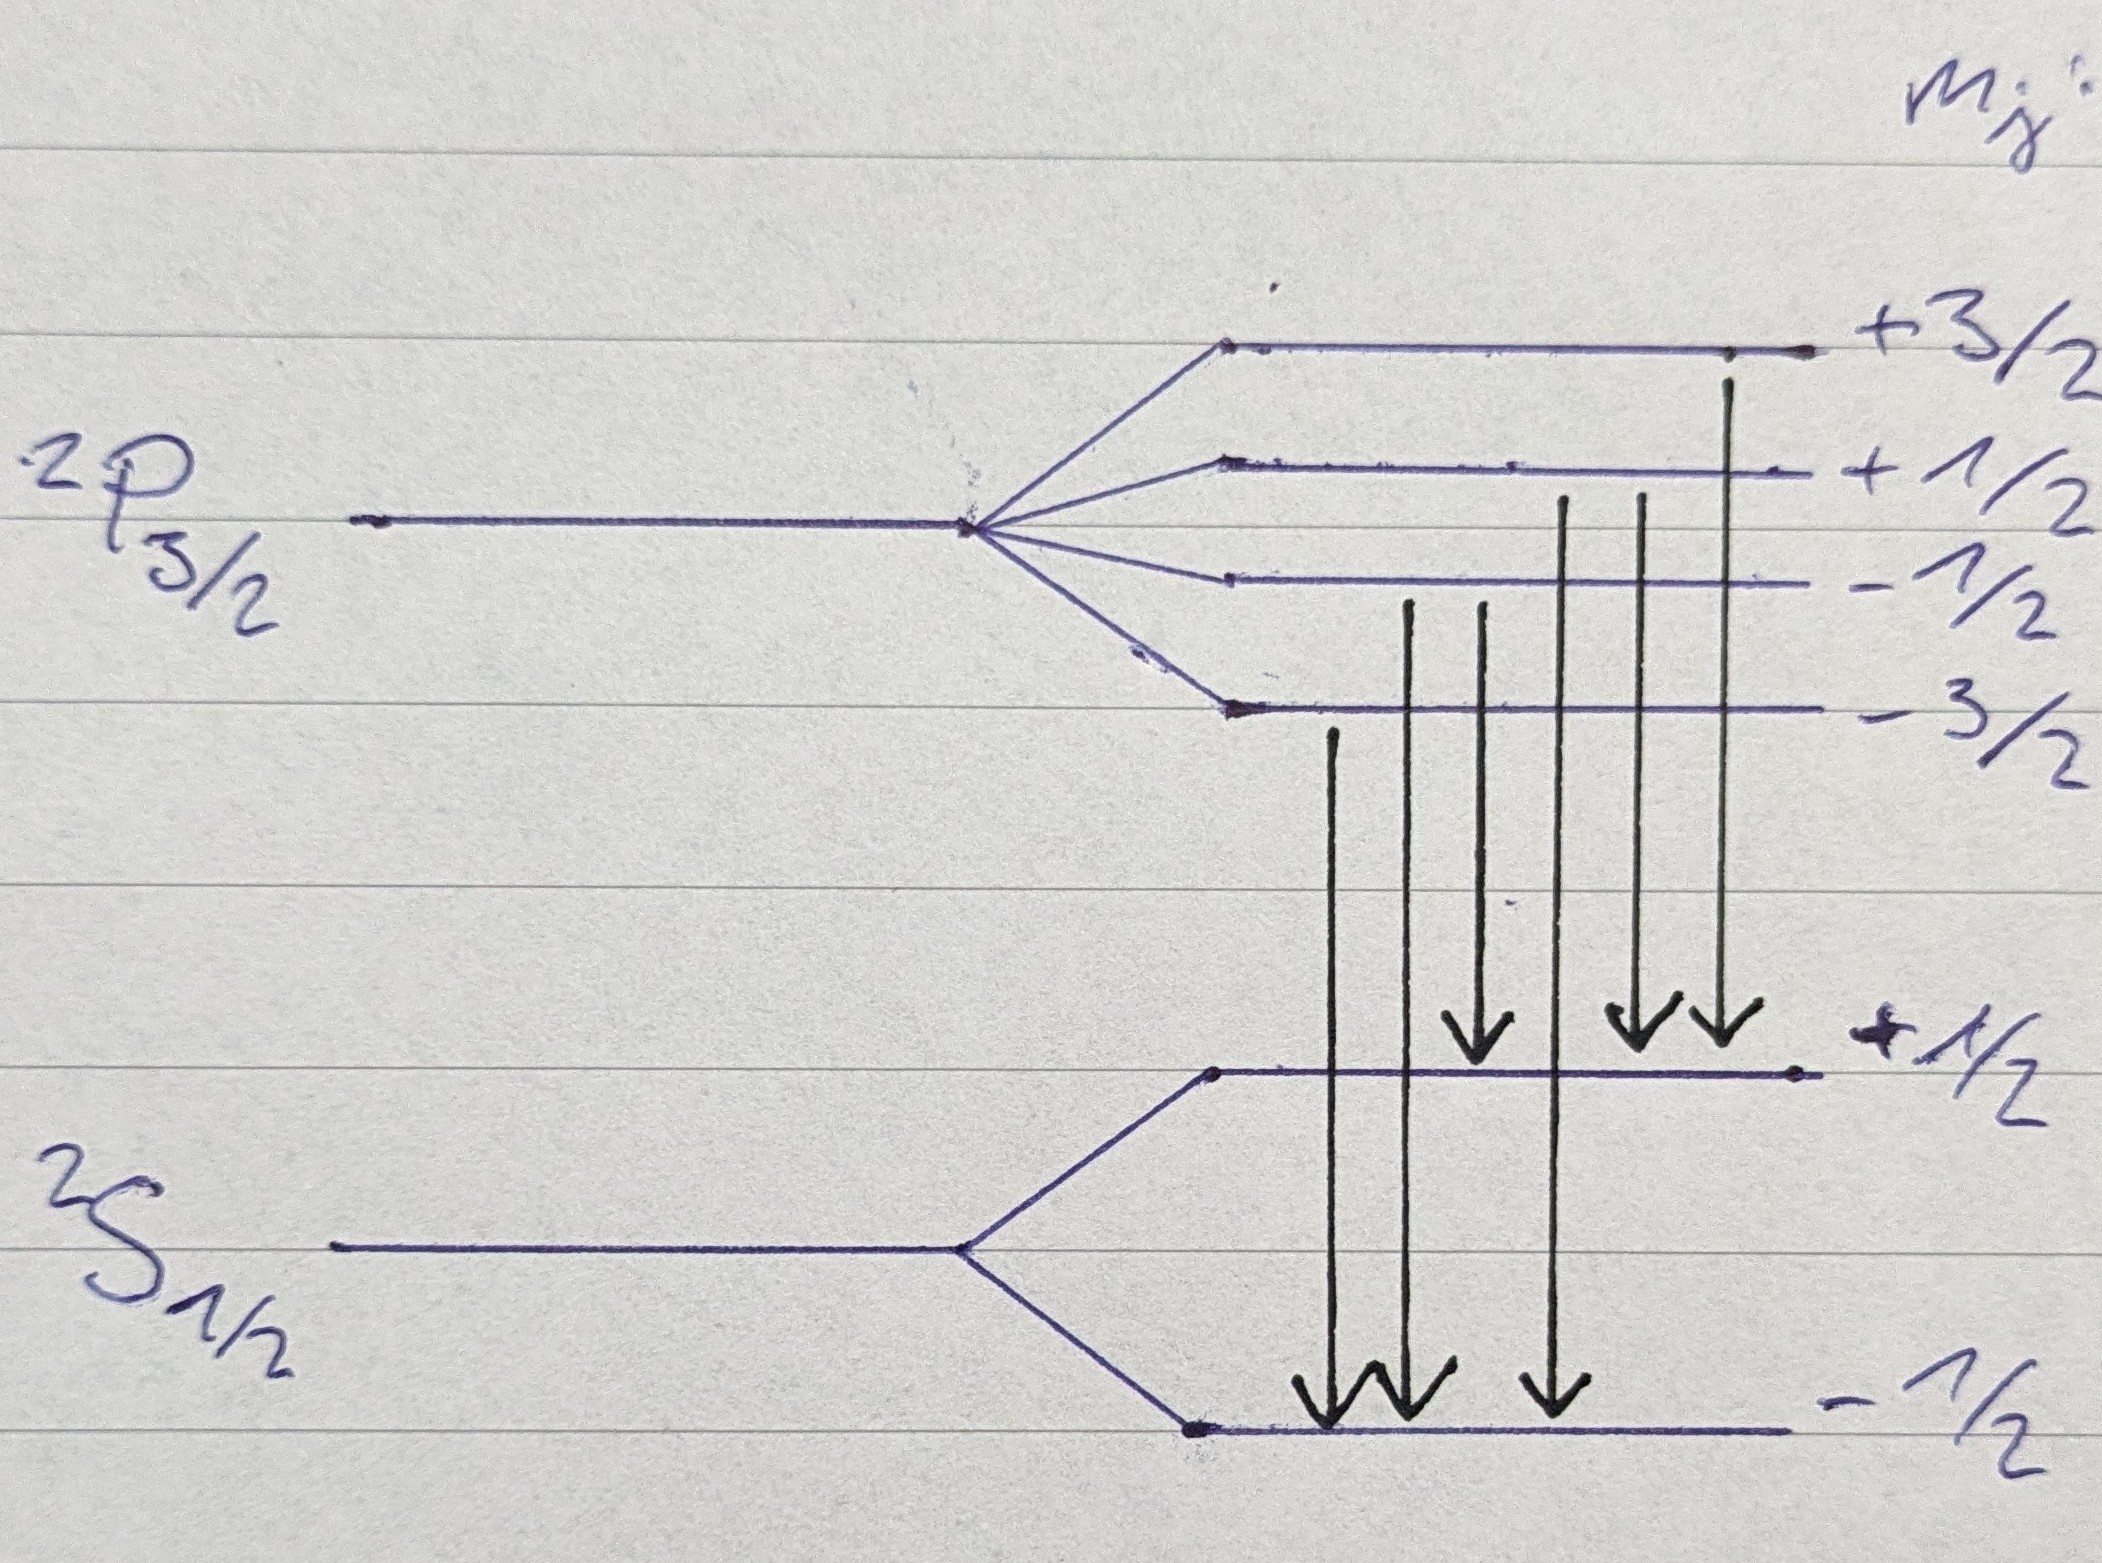
\includegraphics[width=\textwidth]{diagram.jpg}
    \caption{Skizze der Aufspaltung und möglicher Übergänge}
\end{figure}
\end{document}